% Presentation NUMA22 - Lund University
% VT 2015
% (C) Johan Astborg, joastbg@gmail.com
%

\documentclass{beamer}

%\usetheme{AnnArbor}
%\usetheme{Antibes}
%\usetheme{Bergen}
%\usetheme{Berkeley}
%\usetheme{Berlin}
%\usetheme{Boadilla}
%\usetheme{boxes}
\usetheme{CambridgeUS}
%\usetheme{Copenhagen}
%\usetheme{Darmstadt}
%\usetheme{default}
%\usetheme{Frankfurt}
%\usetheme{Goettingen}
%\usetheme{Hannover}
%\usetheme{Ilmenau}
%\usetheme{JuanLesPins}
%\usetheme{Luebeck}
%\usetheme{Madrid}
%\usetheme{Malmoe}
%\usetheme{Marburg}
%\usetheme{Montpellier}
%\usetheme{PaloAlto}
%\usetheme{Pittsburgh}
%\usetheme{Rochester}
%\usetheme{Singapore}
%\usetheme{Szeged}
%\usetheme{Warsaw}

\usepackage{tikz}
\usepackage{pdfpages}
\usepackage[utf8]{inputenc}
\usepackage{listings}
\setbeamercolor{title}{bg=red!65!black,fg=white}

\title{Singular Value Decomposition}

%\subtitle{Project course using Python}

\author{Johan Astborg}

\institute[Lund University]{Computational Programming with Python}

\date{Project Presentation, May 2015}

\subject{The Hydrogen Atom}

\AtBeginSubsection[]
{
  \begin{frame}<beamer>{Outline}
    \tableofcontents[currentsection,currentsubsection]
  \end{frame}
}


\begin{document}

\begin{frame}
  \titlepage
\end{frame}

\begin{frame}{Outline}
  \tableofcontents
\end{frame}

\section{Motivation}
\section{Theory}
\section{The project}

%%%%%%%%%%%%%%%%%%%%%%%%%%%%%%%%%%%%%%%%%%%%

\begin{frame}{Motivation}

\frametitle{Motivation}
\framesubtitle{Matrix decomposition}
%\section{Matrix decomposition}

Consider the matrix $A$
\begin{equation}
A = \begin{bmatrix}4 & 11 & 14 \\8 & 7 & -2 \end{bmatrix}.
\end{equation}

Because $A$ is \emph{singular}, the following eigendecomposition
\begin{equation}
A=VDV^T
\end{equation}
is inapplicable\footnote{Clearly, since $A$ is non-invertible}.

\end{frame}

%%%%%%%%%%%%%%%%%%%%%%%%%%%%%%%%%%%%%%%%%%%%

\begin{frame}{Motivation}

\frametitle{Motivation}
%\framesubtitle{continued}
\framesubtitle{Matrix decomposition cont.}
%\section{Matrix decomposition}

Instead there is a non-trivial possibility, using the absolute values of the eigenvalues instead
\begin{equation}
A=UDV^* .
\end{equation}
These are the \emph{singular values} of $A$, where $A^*$ is \emph{conjugate transpose}.

\end{frame}

%%%%%%%%%%%%%%%%%%%%%%%%%%%%%%%%%%%%%%%%%%%%

\begin{frame}{Motivation}

\frametitle{Motivation}
%\framesubtitle{continued}
\framesubtitle{Geometric representation}
%\section{Matrix decomposition}

\begin{figure}[h] \centering{
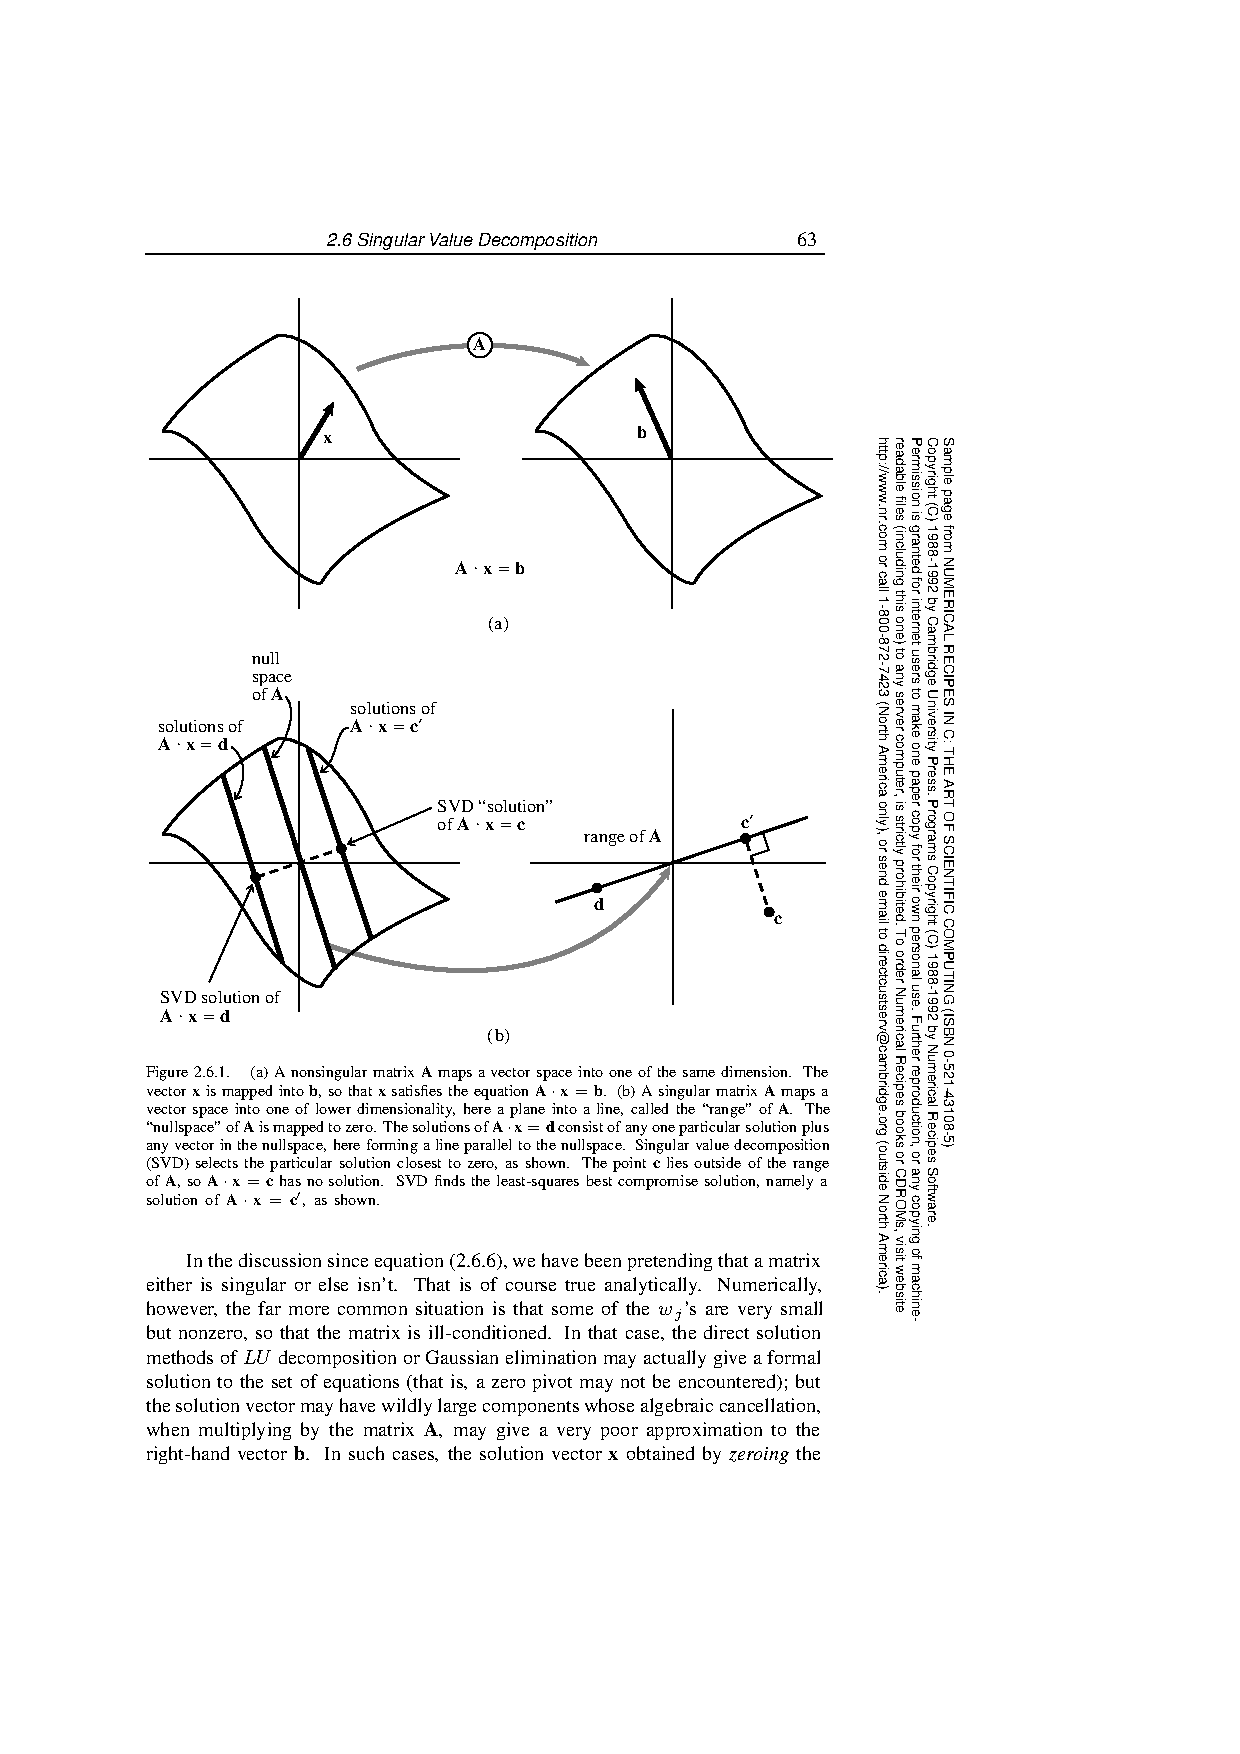
\includegraphics[trim = 20mm 190mm 70mm 210mm, clip=true, scale=0.62]{svd.pdf}}
\end{figure}  


\end{frame}

%%%%%%%%%%%%%%%%%%%%%%%%%%%%%%%%%%%%%%%%%%%%
\begin{frame}
\frametitle{Power Utility Portfolio Choice}

\begin{itemize}
    \item Portfolio Return
        \tikz[remember picture, overlay, baseline=-.5ex]\node (n1) {};
\end{itemize}

\begin{equation*}
\begin{aligned}
& \underset{\boldsymbol w_t}{\text{maximise}}
& & \tikz[baseline,remember picture]{
        \node[fill=blue!20,anchor=base] (t1)
            {$\boldsymbol w_t \cdot \bar{\boldsymbol r}_t $};
    } + \frac{1 - \gamma}{2} 
    \tikz[baseline,remember picture]{
            \node[fill=red!20,anchor=base] (t2)
            {$ \boldsymbol w_t \cdot (\Sigma_t\boldsymbol w_t) $};
    } \\
& \text{subject to}
& & \boldsymbol w_t \cdot \boldsymbol \iota = 1\\
&&& \boldsymbol w_t \ge 0
\end{aligned}
\end{equation*}

\begin{itemize}
    \item Portfolio Variance
        \tikz[remember picture,overlay, baseline=-.5ex]\node (n2) {};
\end{itemize}

\begin{tikzpicture}[remember picture,overlay]
        \path[-stealth] (n1) edge [bend left] (t1);
        \path[-stealth] (n2) edge [out=0, in=-90] (t2);
\end{tikzpicture}

\end{frame}
%%%%%%%%%%%%%%%%%%%%%%%%%%%%%%%%%%%%%%%%%%%%

\begin{frame}{Motivation}

\frametitle{Motivation}
%\framesubtitle{continued}
\framesubtitle{Geometric representation}
%\section{Matrix decomposition}

\begin{equation*}
\begin{aligned}
\sigma_1 & = & \sqrt{360} = 6\sqrt{10} \\
\sigma_2 & = & \sqrt{90} = 3\sqrt{10} \\
\sigma_3 & = & 0
\end{aligned}
\end{equation*}

\end{frame}

%%%%%%%%%%%%%%%%%%%%%%%%%%%%%%%%%%%%%%%%%%%%

\begin{frame}{Motivation}

\frametitle{Motivation}
%\framesubtitle{continued}
\framesubtitle{Geometric interpretation of singular values}
%\section{Matrix decomposition}

First two singular values of $A$ are the length of the semiaxis
of the ellipse (Fig 2).

\end{frame}

%%%%%%%%%%%%%%%%%%%%%%%%%%%%%%%%%%%%%%%%%%%%

\begin{frame}{Definition}

\frametitle{Definition}
%\framesubtitle{continued}
\framesubtitle{Singular Value Decomposition}
%\section{Matrix decomposition}

\begin{equation}
\Sigma = \begin{bmatrix}D & 0 \\ 0 & 0 \end{bmatrix}.
\end{equation}

\end{frame}

%%%%%%%%%%%%%%%%%%%%%%%%%%%%%%%%%%%%%%%%%%%%

\begin{frame}{Theorem}

\frametitle{Theorem}
%\framesubtitle{continued}
\framesubtitle{Singular Value Decomposition}
%\section{Matrix decomposition}

\begin{equation}
A = U\Sigma V^*
\end{equation}
where $U$, $V$ are orthogonal and its positive diagonal
entries is called the \emph{SVD} of $A$.

\end{frame}

%%%%%%%%%%%%%%%%%%%%%%%%%%%%%%%%%%%%%%%%%%%%

\begin{frame}{Proof}

\frametitle{Proof}
\framesubtitle{Singular Value Decomposition}

... since $V$ is orthogonal matrix, $U\Sigma V^* = AUV^T = A$

\end{frame}

%%%%%%%%%%%%%%%%%%%%%%%%%%%%%%%%%%%%%%%%%%%%

\begin{frame}{The Project}

\frametitle{The Project}
\framesubtitle{Singular Value Decomposition}

Implement this in Python given constraints and a set of tasks.

\end{frame}

%%%%%%%%%%%%%%%%%%%%%%%%%%%%%%%%%%%%%%%%%%%%

\begin{frame}{The Project}

\frametitle{The Project}
\framesubtitle{Singular Value Decomposition}

In theory we can follow the following steps
\begin{enumerate}
\item Find the orthogonal dianonalization of $A^T A$
\item Set up $V$ and $\Sigma$
\item Construct $U$
\item Check singular values against eigenvalues ($||Av_i|| = \sigma_i $)
\end{enumerate}

\end{frame}

%%%%%%%%%%%%%%%%%%%%%%%%%%%%%%%%%%%%%%%%%%%%

\begin{frame}{The Project}

\frametitle{Reality check}
\framesubtitle{Singular Value Decomposition}

\textbf{But numerical linear algebra is reality}\\...which means \emph{IEEE-754} and
64-bit FPUs.

\end{frame}

%%%%%%%%%%%%%%%%%%%%%%%%%%%%%%%%%%%%%%%%%%%%

\begin{frame}{The Project}

\frametitle{Reality check}
\framesubtitle{Singular Value Decomposition}

you've seen this \emph{too many times} but here it is again

\end{frame}

%%%%%%%%%%%%%%%%%%%%%%%%%%%%%%%%%%%%%%%%%%%%

\begin{frame}{The Project}

\frametitle{The Project}
\framesubtitle{Requirements}

Requirements for the project
\begin{enumerate}
\item 1
\item 2
\item 3
\item 4
\end{enumerate}

\end{frame}

%%%%%%%%%%%%%%%%%%%%%%%%%%%%%%%%%%%%%%%%%%%%

\begin{frame}{The Project}

\frametitle{The Project}
\framesubtitle{Overview of numerical algorithms}

Overview of algorithms for SVD implementation
\begin{enumerate}
\item 1
\item 2
\item 3
\item 4
\end{enumerate}

\end{frame}

%%%%%%%%%%%%%%%%%%%%%%%%%%%%%%%%%%%%%%%%%%%%

\begin{frame}{The Project}

\frametitle{The Project}
\framesubtitle{The algorithm used}

\textbf{Motivation}:\\ Suggested in the project description\footnote{checked some references anyhow}
\end{frame}

%%%%%%%%%%%%%%%%%%%%%%%%%%%%%%%%%%%%%%%%%%%%

\begin{frame}{The Project}

\frametitle{The Project}
\framesubtitle{Implementation}

\textbf{How it was done}
\begin{enumerate}
\item Paper and pen before thinking code
\item Just a few keystrokes, i.e. Python is a reduced \emph{Lisp}
\item Emacs
\item MATLAB (as a reference)
\end{enumerate}


\end{frame}

%%%%%%%%%%%%%%%%%%%%%%%%%%%%%%%%%%%%%%%%%%%%

\begin{frame}{The Project}

\frametitle{The Project}
\framesubtitle{Challenges}

Yes, \textbf{software development} plus \textbf{numerical analysis} is 
\begin{itemize}
\item A fruitful combination full of surprises
\item Not that bad if you unplug and read some books first
\end{itemize}

\end{frame}

%%%%%%%%%%%%%%%%%%%%%%%%%%%%%%%%%%%%%%%%%%%%

\begin{frame}{The Project}

\frametitle{The Project}
\framesubtitle{Challenges}

\textbf{Not just one thing remains}:\\
Actually appreciate and find use for the final software\footnote{The theory is clear enough}

\end{frame}

%%%%%%%%%%%%%%%%%%%%%%%%%%%%%%%%%%%%%%%%%%%%

\begin{frame}{The Project}

\frametitle{The Project}
\framesubtitle{Checkout the source\footnote{The code will be there soon}}

\begin{center}
\texttt{http://github.com/josatbg/python-svd}
\end{center}

\end{frame}

%%%%%%%%%%%%%%%%%%%%%%%%%%%%%%%%%%%%%%%%%%%%

\begin{frame}{The Project}

\frametitle{The Project}
\framesubtitle{Thanks and have a nice summer}

\begin{center}
\textbf{Thanks!}
\end{center}

\end{frame}

%%%%%%%%%%%%%%%%%%%%%%%%%%%%%%%%%%%%%%%%%%%%


\end{document}



